\subsection{Feature-Redundancy Sensitivity of the Mixed Disease-Associated Signal}
\label{sec:appendix:minimal_panel}

We asked how many of the 293 aptamers preserve the observed within-cohort
disease-associated result. Because biological and technical sources are not
identifiable, this section characterizes feature redundancy of a mixed signal;
it does not validate a reduced assay, clinical deployment, or biomarker panel.
Patient-Stable Aptamer Selection
(PSAS) denotes the fold-specific ranking and development-only budget-selection
protocol below; ``stable'' refers to comparison of ranks across outer folds,
not to equal-patient-weight fitting of the LR ranker.

\noindent\fbox{\begin{minipage}{0.96\linewidth}
\small
\textbf{Algorithm 1: PSAS within outer fold $o$.}
\begin{enumerate}
    \setlength{\itemsep}{1pt}
    \setlength{\parskip}{0pt}
    \item Seal the eight outer-test patients; denote the other 32 patients by $D_o$.
    \item Using all cells in $D_o$, fit development-only standardization and an L1-regularized six-class multinomial LR (SAGA, $C=0.1$); rank aptamer $j$ by $s_j=\sum_{d=1}^{6}|\beta_{dj}|$.
    \item Seed-shuffle the patients in $D_o$ into five patient-disjoint, non-stratified inner folds.
    \item For every $B\in\{5,10,20,40,80,160,293\}$ and inner fold, refit LR on the inner-training patients using the fixed Top-$B$ ranking and score patient-majority-vote macro-F1 on inner-validation patients.
    \item Let $\bar F_B$ denote mean inner-validation macro-F1 and select $B^*=\min\{B:\bar F_B\geq\bar F_{293}-\delta\}$ with $\delta=0.02$.
    \item Refit LR and XGBoost from scratch on all patients in $D_o$, using only the LR-selected Top-$B^*$ features, and evaluate once on the sealed outer-test patients.
    \item Repeat independently for all five outer folds; report the pooled outer-test predictions.
\end{enumerate}
\end{minipage}}
\par\vspace{4pt}

\noindent\textbf{Implementation scope and controls.}
The LR ranker is a cell-level disease model: cells are not first aggregated to
patient medians and receive equal weight, so its coefficients are cell-count
weighted rather than equal-patient-weighted. The full-panel reference $\bar F_{293}$
is the mean inner-validation score, not a resubstitution estimate on all of
$D_o$. The absolute margin $\delta=0.02$ was fixed in code before outer-test
scoring but was not prospectively preregistered. Because the ranking is computed
once from all of $D_o$ and then held fixed across its inner folds, budget
selection is development-only but conditional on that ranking, not fully nested
inner re-ranking.

For Random-$B$, each $B\in\{5,10,20\}$ has 100 uniformly sampled feature sets.
The feature set for one repeat is shared across the five outer folds, but LR and
XGBoost are trained from scratch within every fold. XGBoost in
Table~\ref{tab:panel_budget} and Figure~\ref{fig:panel_curve_main} uses the
LR-selected panel. The separate SHAP control instead fits full-panel XGBoost in
each outer-development set, constructs an equal-patient-weight mean absolute
TreeSHAP ranking, and refits both classifiers on SHAP-selected Top-10/20
features; it does not determine $B^*$ or the main curve.

All five outer folds select $B^*=10$ under this rule.

\begin{figure}[tb]
\centering
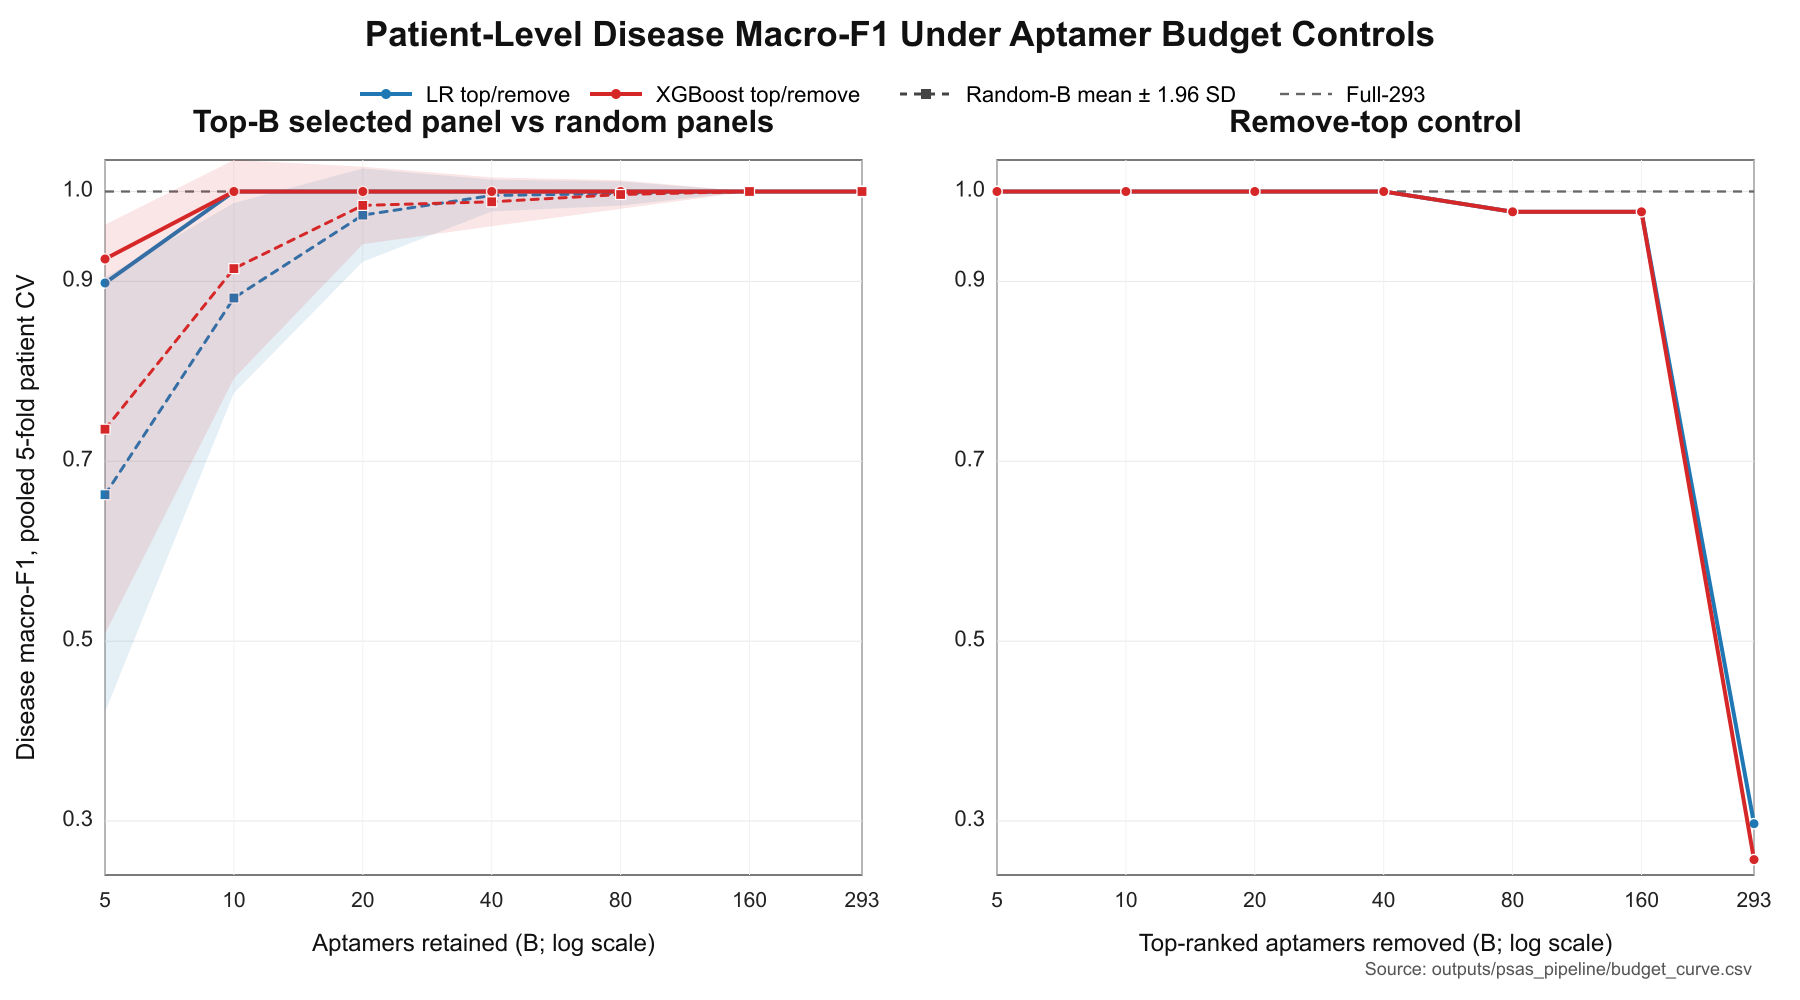
\includegraphics[width=\columnwidth]{figures/panel_size_curve.png}
\caption{
Patient-level disease-association macro-F1 under feature-budget controls. Solid
lines show pooled out-of-fold performance obtained using fold-specific Top-$B$
panels; dotted lines and ribbons show the mean and empirical 95\% interval over
100 random-panel repeats. Each repeat shares one panel across outer folds, with
models refit foldwise. The dashed line is the full 293-aptamer reference; scores
pool the 40 outer-test patients once each.
Because acquisition effects are unrecorded, the curves quantify redundancy of
the mixed within-cohort signal rather than reduced-assay validity.
}
\label{fig:panel_curve_main}
\end{figure}

\par\vspace{4pt}
\noindent\textbf{Budget terminology.}
An \emph{aptamer measurement budget} $B$ means that a model is retrained and evaluated using only those $B$ input features. An \emph{inference-time cell budget} $C$ means that, after training on all available outer-development cells, only $C$ cached predictions are sampled from each held-out patient before majority-vote aggregation. We do not reduce or evaluate a \emph{training-time cell budget}; the cell-count sensitivity therefore supports low-cell inference aggregation, not training with only $C$ cells per patient.

The resulting development-selected 10-aptamer panels reproduce the full-panel patient-level macro-F1 of 1.0 for both Logistic Regression and XGBoost on all five outer test folds. Figure~\ref{fig:panel_curve_main} compares these selected panels with 100 Random-$B$ repeats at each compact budget. For every model and budget, we report the random-panel mean, empirical 2.5th--97.5th percentile interval, and the empirical midrank percentile of Top-$B$ within that distribution (Table~\ref{tab:psas_random}).

\begin{table}[H]
\centering
\small
\setlength{\tabcolsep}{6pt}
\renewcommand{\arraystretch}{1.10}

\begin{tabular}{ccccc}
\toprule
\textbf{Outer Fold} & \textbf{$\delta$} & \textbf{$B^*$} & \textbf{LR Macro-F1} & \textbf{XGBoost Macro-F1} \\
\midrule
0 & 0.02 & 10 & 1.000 & 1.000 \\
1 & 0.02 & 10 & 1.000 & 1.000 \\
2 & 0.02 & 10 & 1.000 & 1.000 \\
3 & 0.02 & 10 & 1.000 & 1.000 \\
4 & 0.02 & 10 & 1.000 & 1.000 \\
\midrule
\textbf{All folds} & \textbf{0.02} & \textbf{10} & \textbf{1.000} & \textbf{1.000} \\
\bottomrule
\end{tabular}

\caption{
Outer-test-isolated feature-budget sensitivity for the mixed disease-associated signal. In each
outer fold, aptamer ranking and budget selection are performed using
outer-development patients only, and the selected budget is evaluated once on
the untouched outer-test patients. The ranking is fixed across inner validation
splits; $B$ is selected conditional on that ranking. Under the analysis-specified,
non-preregistered tolerance margin $\delta=0.02$, all five folds select the same development budget
$B^*=10$, and the resulting 10-aptamer panels preserve the observed
full-panel patient macro-F1 for both Logistic Regression and XGBoost.
This result demonstrates feature redundancy of the observed mixed
disease-associated signal. It does not validate a reduced assay, a biological
signature, or unique causal biomarkers.
}
\label{tab:panel_budget}

\end{table}


\begin{table}[t]
\centering
\scriptsize
\setlength{\tabcolsep}{3pt}
\begin{tabular}{cclcc}
\toprule
$B$ & Model & Top-$B$ & Random mean [95\% interval] & Percentile \\
\midrule
5 & LR & 0.898 & 0.663 [0.422, 0.890] & 97.0 \\
5 & XGBoost & 0.925 & 0.725 [0.453, 0.890] & 99.0 \\
10 & LR & 1.000 & 0.868 [0.670, 0.952] & 100.0 \\
10 & XGBoost & 1.000 & 0.921 [0.781, 1.000] & 97.0 \\
20 & LR & 1.000 & 0.973 [0.900, 1.000] & 79.5 \\
20 & XGBoost & 1.000 & 0.981 [0.923, 1.000] & 75.0 \\
\bottomrule
\end{tabular}
\caption{Compact-panel random controls over 100 independently sampled panels. Top-$B$ uses a fold-specific LR ranking fitted only on outer-training patients. The percentile uses the empirical midrank of Top-$B$ within the random distribution.}
\label{tab:psas_random}
\end{table}


At $B=10$, the Top-$B$ panel is at the 100th empirical percentile for LR and the 97th for XGBoost; Random-$B$ means are 0.868 and 0.921, respectively. By $B=20$, random means rise to 0.973 and 0.981 and many random panels also saturate, reducing the corresponding midrank percentiles to 79.5 and 75.0. Thus ranking is most consequential at the smallest budgets, while the broader panel contains extensive substitutable signal.

We next crossed aptamer budget $B\in\{5,10,20,293\}$ with inference-time cell caps $C\in\{100,500,1000,5000,\mathrm{all}\}$. For each finite cap, cached predictions were sampled without replacement within each outer-test patient; patient majority votes were pooled across the five held-out folds, and the process was repeated over 50 sampling seeds. Training still used all outer-development cells. At $B=5$, macro-F1 varies with the sampled cells and reaches 0.881 on average at $C=100$; at $B=10$, $20$, and $293$, macro-F1 is 1.0 for every cap and every seed (Table~\ref{tab:psas_cellcount}).

\begin{table*}[t]
\centering
\scriptsize
\setlength{\tabcolsep}{3pt}
\begin{tabular}{clllll}
\toprule
$B$ & 100 cells & 500 cells & 1,000 cells & 5,000 cells & All cells \\
\midrule
5 & 0.881 [0.845, 0.925] & 0.894 [0.852, 0.925] & 0.906 [0.875, 0.925] & 0.899 [0.898, 0.898] & 0.898 [0.898, 0.898] \\
10 & 1.000 [1.000, 1.000] & 1.000 [1.000, 1.000] & 1.000 [1.000, 1.000] & 1.000 [1.000, 1.000] & 1.000 [1.000, 1.000] \\
20 & 1.000 [1.000, 1.000] & 1.000 [1.000, 1.000] & 1.000 [1.000, 1.000] & 1.000 [1.000, 1.000] & 1.000 [1.000, 1.000] \\
293 & 1.000 [1.000, 1.000] & 1.000 [1.000, 1.000] & 1.000 [1.000, 1.000] & 1.000 [1.000, 1.000] & 1.000 [1.000, 1.000] \\
\bottomrule
\end{tabular}
\caption{LR patient-level macro-F1 under equal-cell subsampling. Entries are mean [empirical 95\% interval] over 50 sampling seeds; predictions are pooled across the five outer test folds before scoring the 40 patients.}
\label{tab:psas_cellcount}
\end{table*}


Finally, we tested whether the compact result depends on Logistic Regression coefficients as the attribution mechanism. Within each outer-development set, we fitted a full-panel XGBoost model and computed absolute TreeSHAP contributions on at most 1,000 cells per development patient. We first averaged over cells within each patient and then over patients, preventing high-cell-count patients from dominating the attribution ranking. The LR--SHAP Jaccard overlap is moderate rather than complete (0.501 for Top-10 and 0.475 for Top-20), yet panels from either ranking achieve patient macro-F1 1.0 when evaluated with either LR or XGBoost (Table~\ref{tab:psas_shap}). This cross-model control supports predictive redundancy of the mixed signal, not measurement efficiency, molecular specificity, or a unique signature.

\begin{table}[H]
\centering
\scriptsize
\setlength{\tabcolsep}{3pt}
\begin{tabular}{cclcc}
\toprule
$B$ & LR--SHAP Jaccard & Ranking & LR eval. & XGB eval. \\
\midrule
10 & 0.501 $\pm$ 0.126 & LR coefficient & 1.000 & 1.000 \\
10 & -- & XGBoost-SHAP & 1.000 & 1.000 \\
20 & 0.475 $\pm$ 0.087 & LR coefficient & 1.000 & 1.000 \\
20 & -- & XGBoost-SHAP & 1.000 & 1.000 \\
\bottomrule
\end{tabular}
\caption{Cross-model attribution control. Jaccard is mean $\pm$ SD across five outer-fold Top-$B$ sets. LR-coefficient and XGBoost-SHAP rows use their own selected features; evaluation columns report pooled patient macro-F1 after refitting LR or XGBoost. SHAP ranking does not select $B^*$.}
\label{tab:psas_shap}
\end{table}


The fold-overlap LR ranking is also stable. The highest-ranked aptamers by mean outer-fold rank are APT-179, APT-225, APT-164, APT-166, APT-57, APT-69, APT-125, APT-161, APT-172, and APT-218, and 290 of the 293 aptamers are retained after a simple redundancy screen at $|r| \le 0.9$. These anonymized IDs have no verified public protein-target mapping, and feature ranking under unresolved confounding cannot support protein-target, pathway, or molecular-plausibility interpretation. We therefore omit the earlier full-cohort attribution visualization.
